\section{\system}

\eat{%
{\system} is a web-based system build on top of the PostgreSQL open 
source database system. Computation for visualization is performed
using HTML, CSS and javascript. Calculations are performed using 
in-database computation through AJAX calls and client side 
javascript. In this section we discuss each part of \system. 
}

{\system} system was built to process large amounts of article,
provide fast response to user queries and display descriptive
results to the user.
In this section we describe our preprocessing steps to extract
topic models from the documents.
We then discuss the User Model behind each user search, we then
discuss our methods for topic-based search and exploration.



\subsection{Data pre-processing and topic learning}

Here we describe the main pre-processing steps we perform on a 
collection of articles for topic modeling and search. First, 
we tokenize raw texts of articles with the help of the python 
Natural Language Toolkit (NLTK)~\footnote{\texttt{http://www.nltk.org/}} and a set of 
predefined regular expressions. Second, we standardize tokens by 
removing noise and stop-words. We use typical standardization 
techniques for word tokens such as \textsl{stemming}---for this 
project, we use the popular Porter stemming algorithm~\cite{Porter1980} 
implementation in NLTK\@. Third, we represent each 
document in a sparse ``bag of words'' format, after building a 
vocabulary of corpus words. Last, we use them as input to the topic 
learning algorithm~\cite{hoffman2010online} which will in turn learn 
the latent topic structure of a corpus from the term co-occurrence 
frequencies of the corresponding documents. Components of a learned 
topic model includes the estimated corpus-level topics, $\beta_j^{*}$s, 
and document-level topic mixtures, $\theta_d^{*}$s. As discussed, 
$\beta_j^{*}$ is useful for our automatic detection of topics among  
articles. Similarly, $\theta_d^{*}$ give an idea of the topicality 
of a particular article given a topic. This is quite useful in 
finding similar articles and grouping them together. In addition, 
topic modeling is a type of dimensionality reduction technique that 
enables us to work on the topic-space rather than on the 
vocabulary-space.



\subsection{User Model}
When performing search, exploration and discovery over academic papers users 
may bring particular context to their search. Incorporating this information
into the search process has been show to be beneficial to 
users~\cite{DZSRWJ,MZPGSOL}.
We develop a user model that 
encapsulates the users personal context and integrates it into their
search task. 

This model is a distribution of weights for each topic.
Formally, given a set of topics $T$ the user model is defined as
$$
\mathcal{U} = \{u_0, \ldots, u_{|T|}\}
$$
where $u_i \in [0,1]$ and $\sum_{t \in T} u_t = 1$.
We graphically allow the user to select the weights that correspond to
each topic. This allows the users to change preferences with each query
for more desirable results.

The user model is used in different ways to provide better feedback to
the user. After a keyword search, the document results of the search 
are re-ranked by calculating the KL-divergence of each document and the
user model. Formally, given the set of result documents $D$:

\begin{equation} \label{eq:KL}
KL(\mathcal{U}||d) = \sum_{t \in T} u_t \ln \frac{u_t}{d_t}.
\end{equation}
where $d \in D$ and $d_t$ is the topic proportion for document $d$ and
topic $t \in T$. 

In the topic explorer, each topic row is color-coded like a heat 
based map based on the similarity of the user model to that topic (see Figure~\ref{fig:topic_exploration}).
The user can look at this heat map to adjust their topic preferences.
We use equation~\ref{eq:KL} on the client side to calculate this preference. 
In the graph explorer the citations for the current paper is ranked
using equation~\ref{eq:KL}. The citations of that paper that are most
similar to the user model are ranked the highest.


\subsection{Topic-Based Search}

\system provides several ranking choices to let the user find  
the best articles. One way of ranking is to identify the topics of 
real interest, by looking at the most \textsl{informative terms} of 
the estimated topics $\beta_j^{*}$ for the corpus, and then 
determine relevant articles given the topic of interest. The 
simplest way to identify informative terms in a topic is to 
determine the most probable words by sorting the vocabulary terms in 
the order of their term probabilities, $\beta_{jt}^{*}$s. In the 
literature, people have looked at several other methods for finding 
informative terms~\cite{2012-termite} and evaluating topics~\cite{mimno2011optimizing}. In this paper, we use a visualization scheme 
developed in~\cite{Davis2013}, for visualizing the most probable 
words in a topic. For example, see Figure~\ref{fig:topic-word-cloud} 
for visualizing a topic which is extracted from a corpus that is 
built from a subset of Wikipedia articles under the category 
\textsl{Whales}. 
       
\begin{figure*}[htb]\centering 
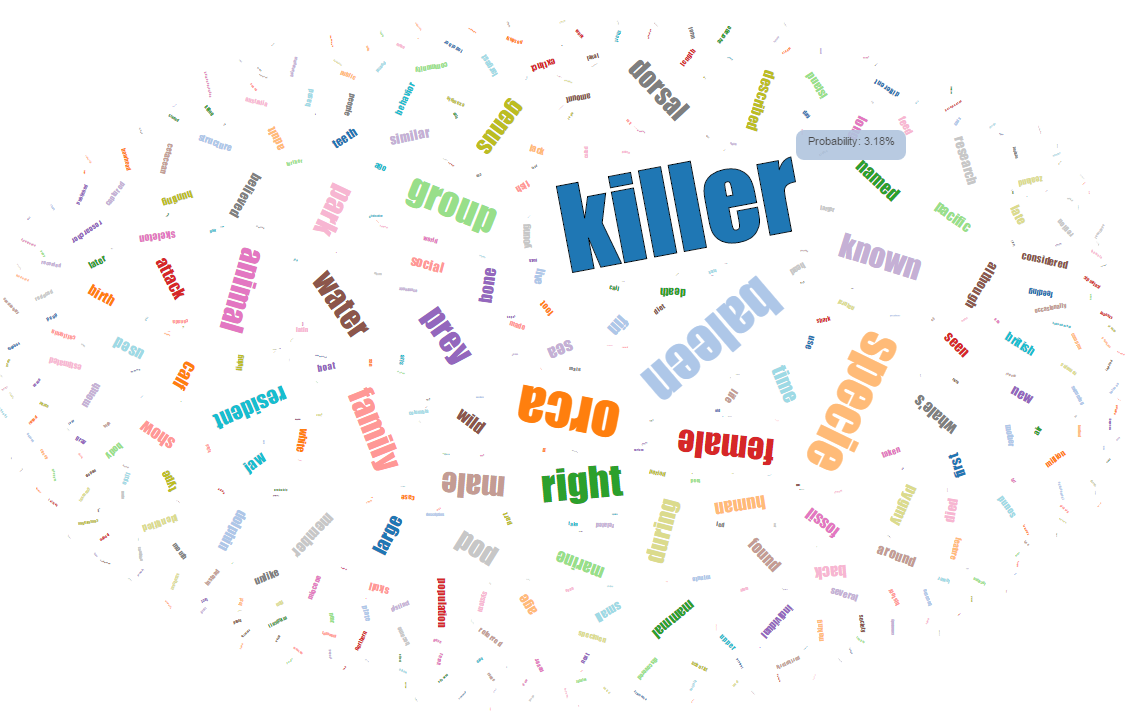
\includegraphics[width=.9\textwidth]{images/topic_visualization.png}
\caption{\textsl{Topic Word Cloud}. Words with high probabilities for the 
given topic are larger in size and words with low probabilities for 
the given topic are smaller in size. From the most probable words, 
we can infer that the topic is mainly refers the Wikipedia category 
\textit{Killer Whales}---one of the main categories from which, we 
downloaded the articles for the corpus.}
\label{fig:topic-word-cloud}
\end{figure*}

We can exploit the estimated document specific topic 
distributions $\theta_d^{*}$s of individual articles, to rank them 
on relevance given a topic. Let $t$ be the index for the topic of 
interest, we calculate~\cite{George2012}
\begin{equation}
m(d) = \ln \theta^*_{dt} + \sum_{j \neq t}{\ln (1 - \theta^*_{dj})}
\end{equation}
for all documents $d = 1, 2, \ldots, D$ in the document collection, 
where $j = 1, 2, \ldots, K$, and sort them to rank them on relevance. 
Here, we assume that each $\theta^*_{dt}$ is normalized, i.e., 
$\sum_{j=1}^{K}{\theta^*_{dj}} = 1$. Intuitively, we can see that 
this equation will give a high value for a document, if the probability 
of occurring topic $t$ is high in that document. This means a 
document with a higher value of this score is highly relevant for 
the topic of interest $t$, and contains a considerable amount of 
words from topic $t$. In the next section, we will see more details 
about \system's visualization methods for the estimated topics and 
ranked documents given a set of estimated topics.      


\noindent\textbf{Topic-Based Exploration and Lineage Search}

Here, we use the estimated document specific topic distribution, 
$\theta^*_{d}$, of an article from the LDA model, for visualizing 
the hidden topical content of the article. For example, Figure~\ref{fig:doc-topic-distribution} shows a visualization based on Pie
Charts\footnote{\texttt{https://developers.google.com/chart}} for 
the $\theta^*_{d}$ of the Wikipedia article \textit{Killer Whale}, 
which is an article listed under the Wikipedia category          
\textit{Killer Whales}. Different slices of the pie chart represents
different topics in the article \textit{Killer Whale} and the size 
of a slice represents the probability of a topic given the article. 
For this illustration, we manually labeled all the topic 
distributions obtained via the LDA posterior inference on a 
corpus---that is built using a subset of Wikipedia articles under the 
category \textit{Whales}---with the help of the topic word clouds 
and the Wikipedia subcategories under the category \textit{Whales}.         
Once we find an interesting topic to pursue, we can explore all 
the relevant documents under that topic based on the method 
described above. 

\begin{figure}[htb]\centering 
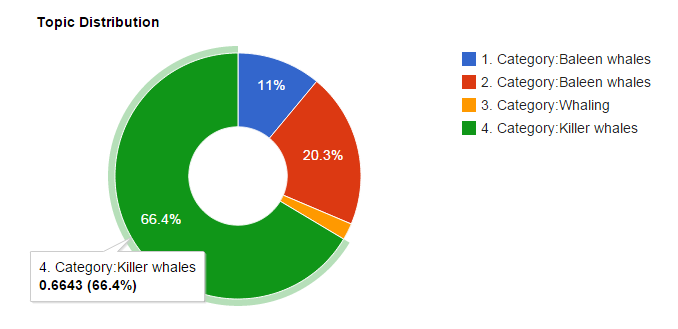
\includegraphics[width=.45\textwidth]{images/doc_topic_distribution.png}
\caption{Visualization of the document specific topic distribution 
for the Wikipedia article \textit{Killer Whale}.}
\label{fig:doc-topic-distribution}
\end{figure}

Another way to visualize a document is to look at its 
\textsl{paragraph} or \textsl{section} specific topic distributions. 
Each section or paragraph is written with careful attention is every 
peer review article or paper. For example, most of the articles in 
Wikipedia follow a style guide. If we look at an article or paper,  
we can easily decide which section or paragraph is of our interest. 
This intuition can be used to improve topic based exploration. We 
the learned LDA model for the corpus for estimating section or 
paragraph's topic distribution using the Gensim LDA implementation 
\cite{rehurek_lrec}. This is an online task and is performed when a 
user selects a section or paragraph of an article, which is 
described in detail in the \system Demonstration section.  


Another interesting option to explore is how we can use an article's 
topic distribution for searching similar articles of interest. 
Recall the LDA model enable us to transform documents in a 
corpus into vectors, e.g., $\theta^*_{d}$s, in a lower dimensional 
topic space. We can then define similarity between documents via any 
typical vector space similarities, e.g.., cosine similarity. In 
\system we call this as article \textsl{lineage search}.         

